%==========================================================
\section{Modelos de trabalho individuais}\label{sec:modelos}


\subsection{Convenções comuns}

\begin{itemize}
  \item Cada modelo individual é desenhado do ponto de vista de \textbf{uma só pessoa} (A0 ou U0).
  \item Só entra no modelo o que foi \textbf{observado} ou contado como \textbf{caso concreto}. Cada elemento cita o registo que o sustenta, por exemplo \reg{UE07}.
  \item O relâmpago \bolt{} marca um \textit{breakdown}.
  \item As setas e anotações usam a linguagem do participante e não termos técnicos da equipa.
  \item Os dados demográficos ficam no perfil (Tabela~\ref{tab:sessoes}) e não nos modelos.
\end{itemize}

Os ficheiros-fonte dos modelos (\texttt{.drawio}) estão no repositório da equipa e publicamente disponíveis em:
\url{https://github.com/TiagoSilva35/Roamly}.

%----------------------------------------------------------
\subsection{Modelos de fluxo}\label{sec:fluxo}

O modelo de fluxo mostra quem faz o quê e com quem coordena: 
pessoas e papéis (com as suas responsabilidades), lugares de coordenação, 
artefactos e comunicações.

\subsubsection{Fluxo de A0: agente de balcão}

\begin{figure}[!htbp]
\centering
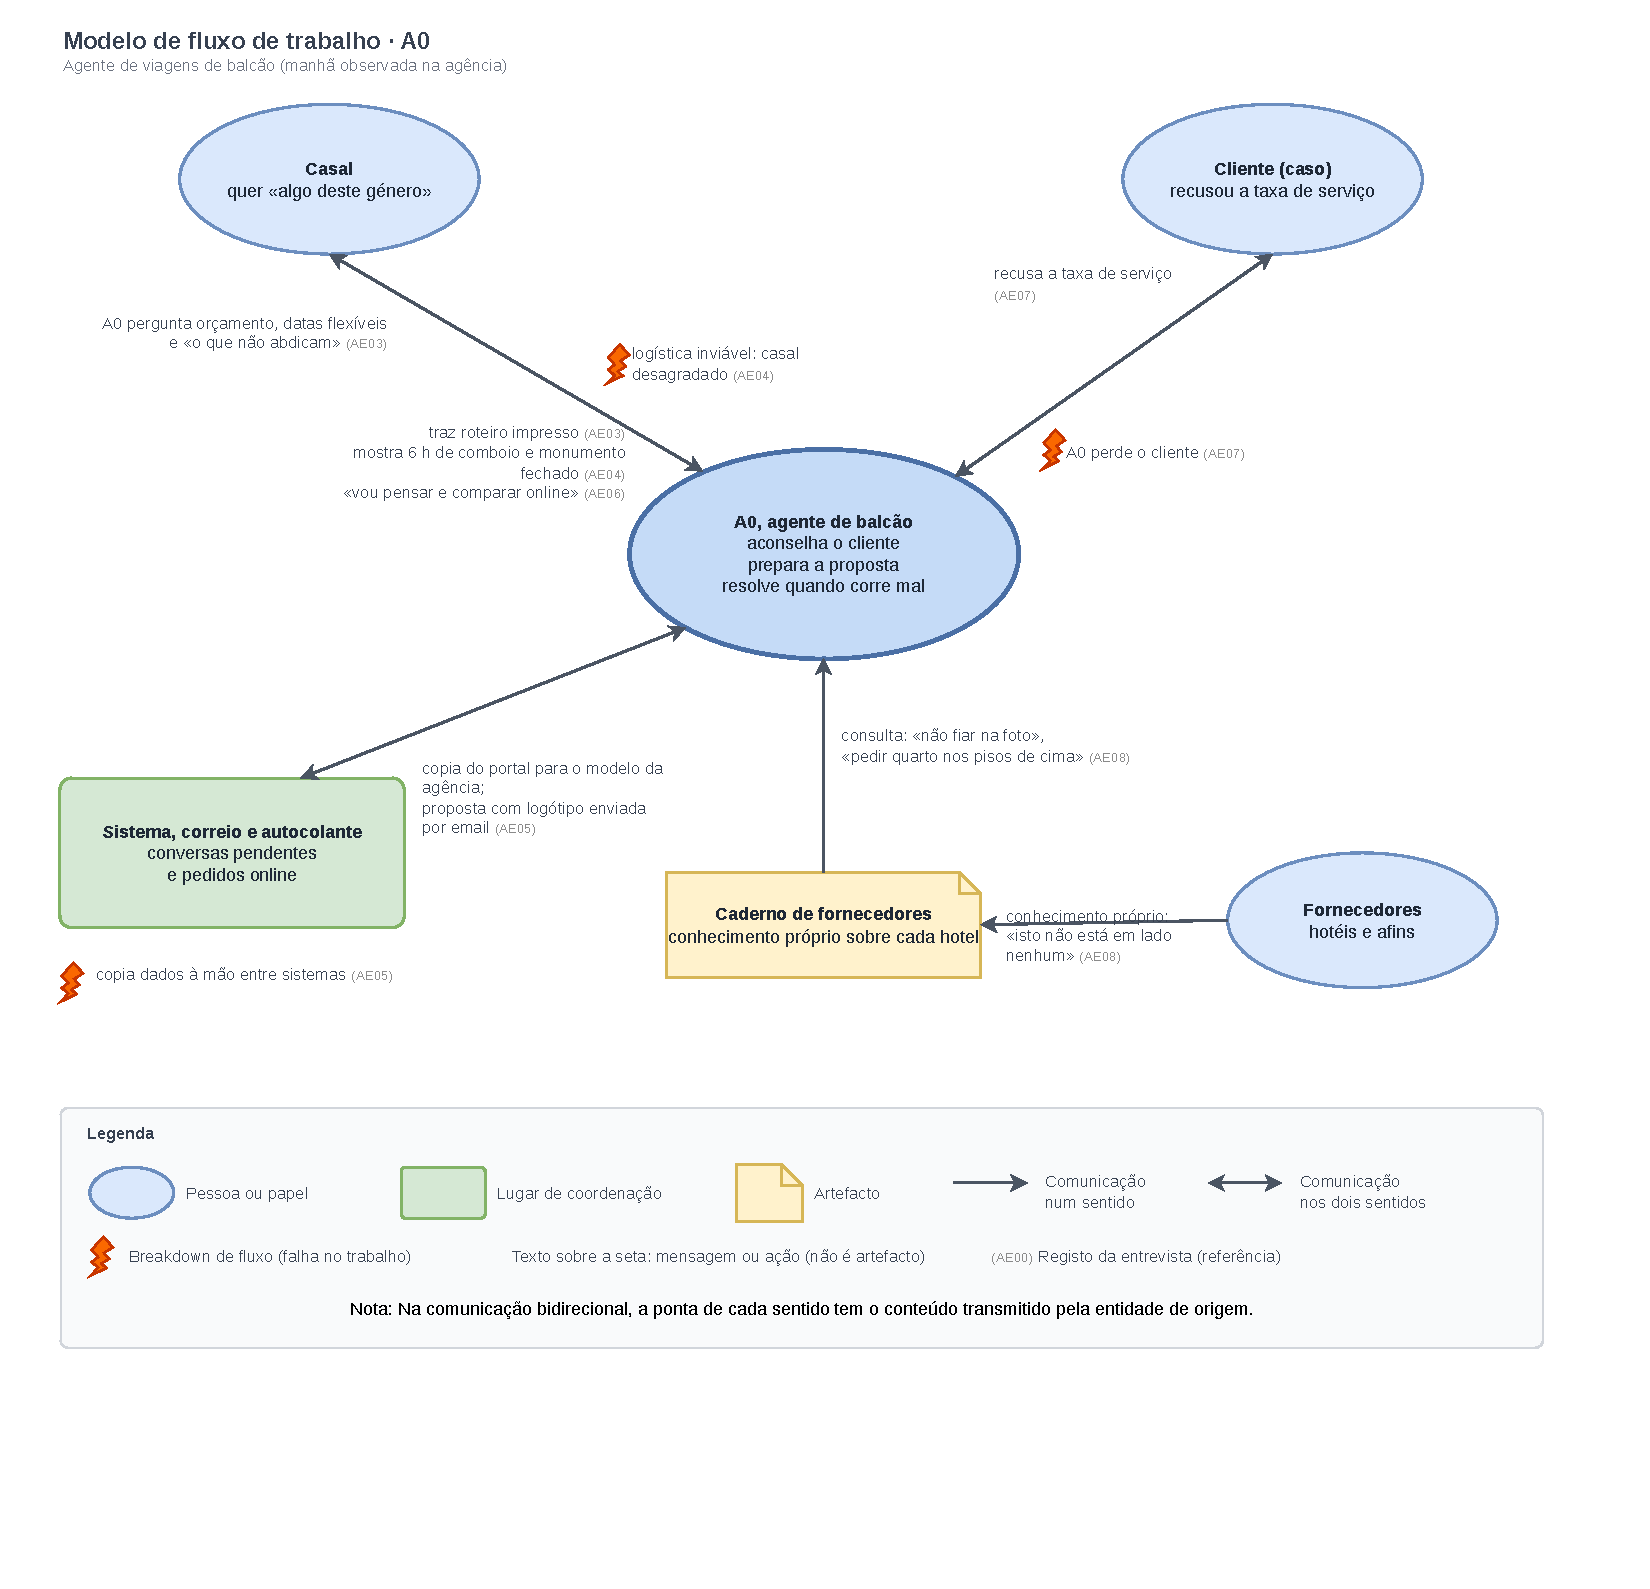
\includegraphics[width=\textwidth]{flow_models/individuais/A0flux.drawio.pdf}
\caption{Modelo de fluxo de A0 (agente de viagens de balcão).}
\label{fig:fluxo-a0}
\end{figure}

A0 está no centro de três frentes. \textbf{Com o cliente presencial} (o casal), 
A0 faz perguntas de descoberta («orçamento, datas flexíveis, o que não abdicam») 
e desfaz um roteiro inviável \reg{AE03, AE04}; o casal leva a proposta e diz que 
vai «pensar e comparar online» \reg{AE06}. \textbf{Com os sistemas da agência} 
(sistema de conversas pendentes, correio partilhado e um papel autocolante no ecrã), 
A0 recebe pedidos e copia à mão os dados do portal para o modelo de proposta da 
agência \reg{AE01, AE05}. \textbf{Com os fornecedores}, A0 recorre a um caderno 
pessoal com conhecimento que «não está em lado nenhum» \reg{AE08}.

\begin{table}[!htbp]
\centering\small
\begin{tabularx}{\textwidth}{@{}p{0.5cm}Lp{2.2cm}@{}}
\toprule
 & \textbf{Breakdown} & \textbf{Registo} \\
\midrule
\bolt & O roteiro do casal tem logística inviável; o casal fica desagradado. & AE04 \\
\bolt & Um cliente recusa a taxa de serviço porque «o site não cobra»; A0 perde-o. & AE07 \\
\bolt & A0 copia dados à mão entre sistemas para montar a proposta. & AE05 \\
\bottomrule
\end{tabularx}
\caption{\textit{Breakdowns} do modelo de fluxo de A0.}
\label{tab:bd-fluxo-a0}
\end{table}

\subsubsection{Fluxo de U0: viajante organizador(a)}

\begin{figure}[!htbp]
\centering
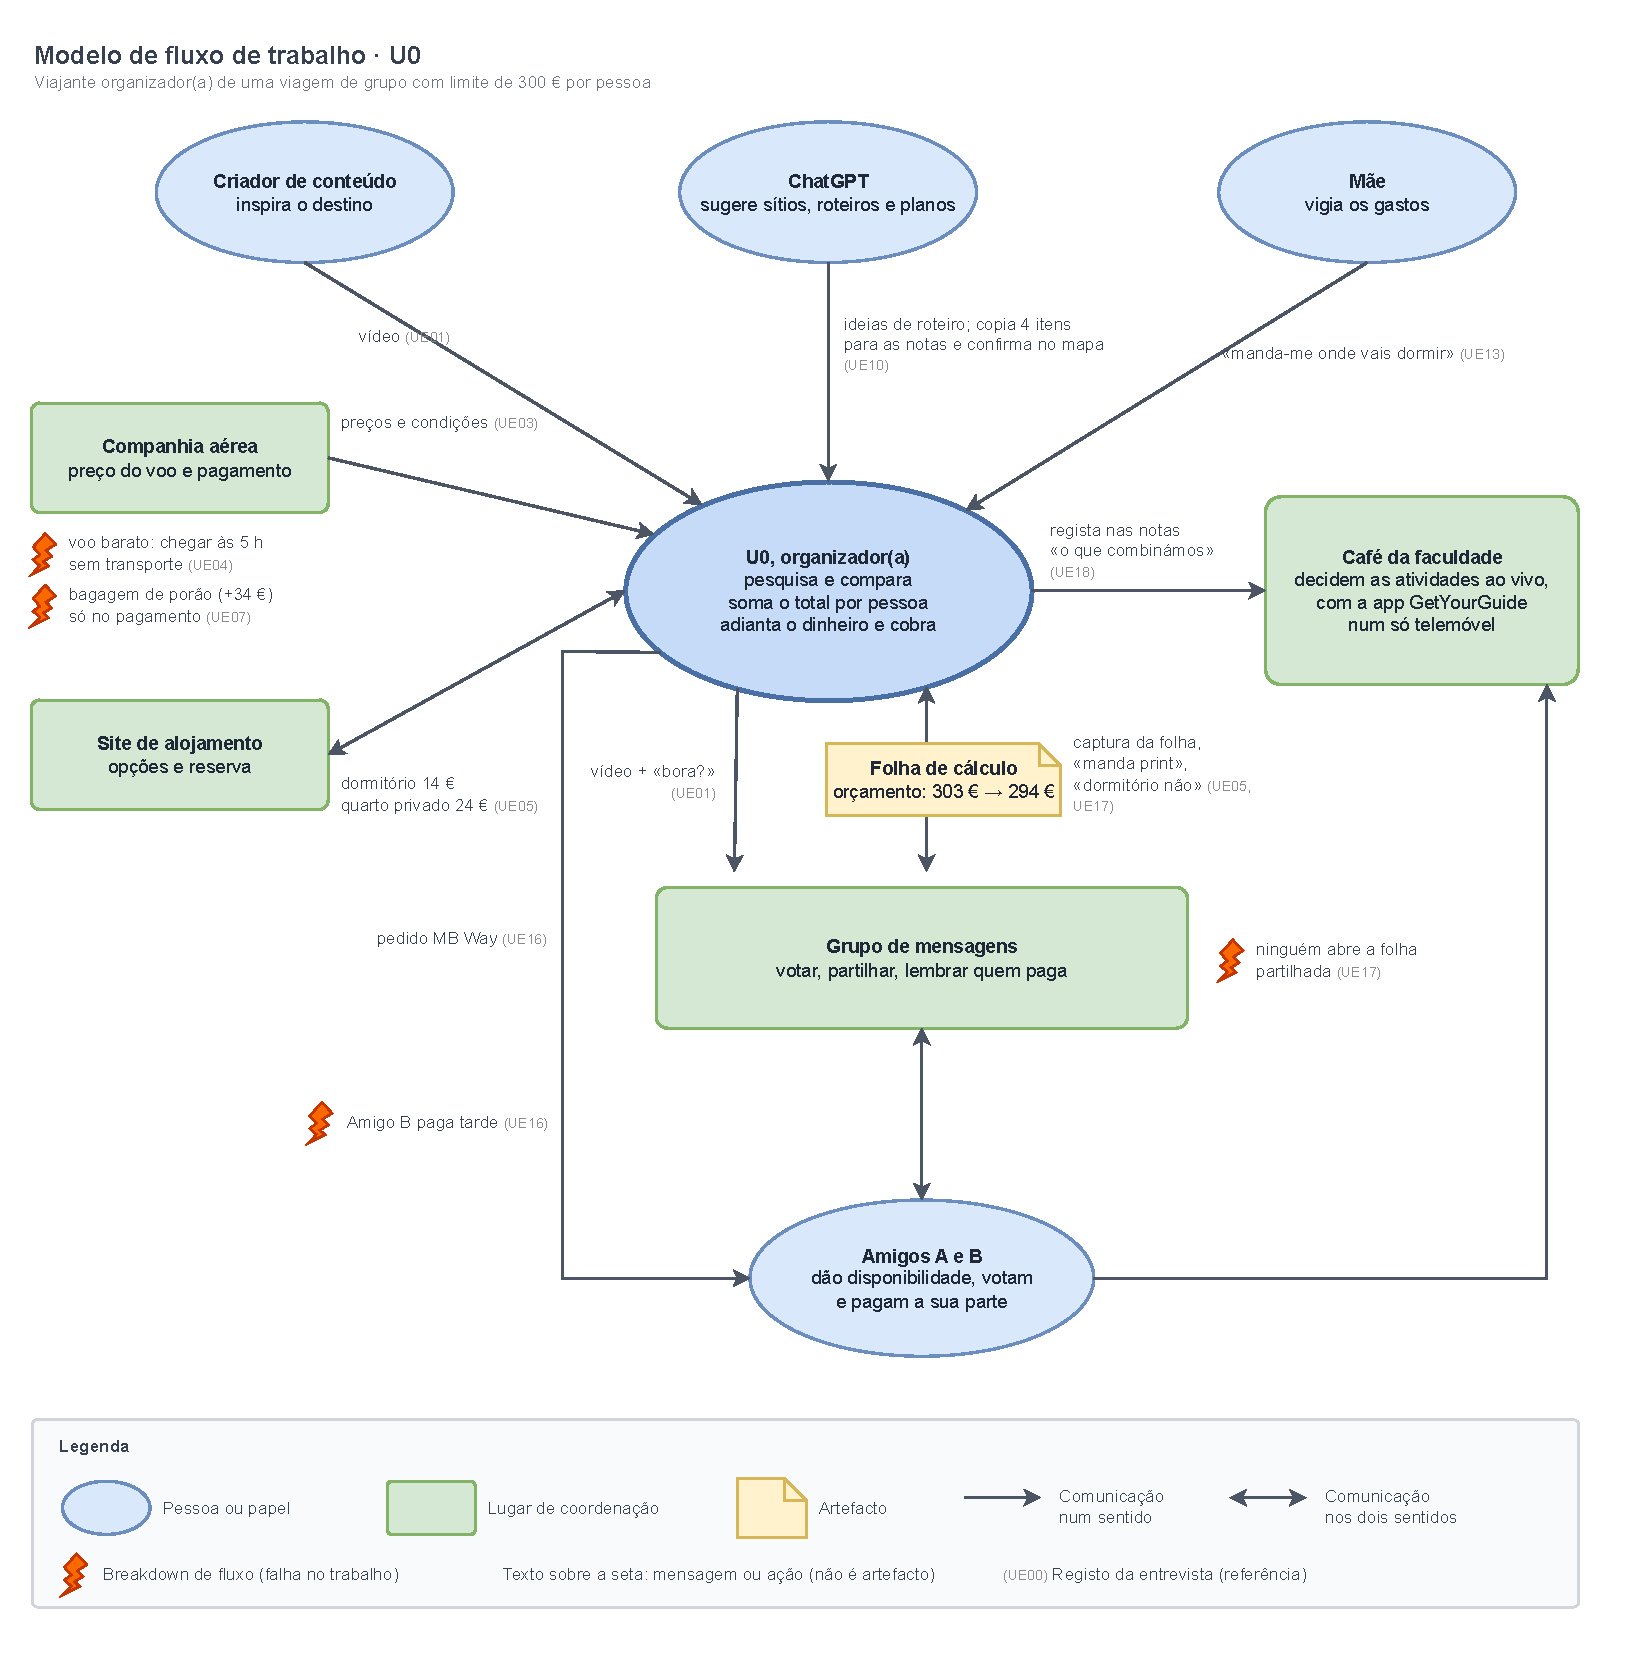
\includegraphics[width=\textwidth]{flow_models/individuais/FluxU0.drawio.pdf}
\caption{Modelo de fluxo de U0 (viajante que organiza uma viagem de grupo).}
\label{fig:fluxo-u0}
\end{figure}

U0 é o ponto por onde passa tudo. A viagem nasce de um vídeo de um 
criador de conteúdo \reg{UE01} e vai ganhando forma com ideias de 
roteiro pedidas ao ChatGPT e confirmadas no mapa \reg{UE10}. U0 
pesquisa sozinho(a) na companhia aérea e no site de alojamento \reg{UE03, UE05} 
e soma tudo numa folha de cálculo que vai de 303\,€ a 294\,€ \reg{UE06, UE12}. 
A coordenação com os amigos passa pelo grupo de mensagens, onde a folha só circula 
como captura de ecrã \reg{UE17}, e pelo café da faculdade, onde as atividades se 
decidem ao vivo num só telemóvel \reg{UE18}. U0 adianta o dinheiro e pede depois a 
parte de cada um \reg{UE16}. A mãe pede para saber onde U0 vai dormir \reg{UE13}.

\begin{table}[!htbp]
\centering\small
\begin{tabularx}{\textwidth}{@{}p{0.5cm}Lp{2.2cm}@{}}
\toprule
 & \textbf{Breakdown} & \textbf{Registo} \\
\midrule
\bolt & O voo barato obriga a chegar ao aeroporto às 5\,h, sem transporte. & UE04 \\
\bolt & A bagagem de porão (+34\,€) só aparece no pagamento. & UE07 \\
\bolt & Ninguém abre a folha partilhada; o grupo pede «print». & UE17 \\
\bolt & O Amigo~B paga tarde. & UE16 \\
\bottomrule
\end{tabularx}
\caption{\textit{Breakdowns} do modelo de fluxo de U0.}
\label{tab:bd-fluxo-u0}
\end{table}

%----------------------------------------------------------
\subsection{Modelos culturais}\label{sec:cultural}

O modelo cultural mostra as pressões, valores e expectativas que condicionam o 
trabalho~\cite{beyer1998}.

\subsubsection{Cultural de A0}

\begin{figure}[!htbp]
\centering
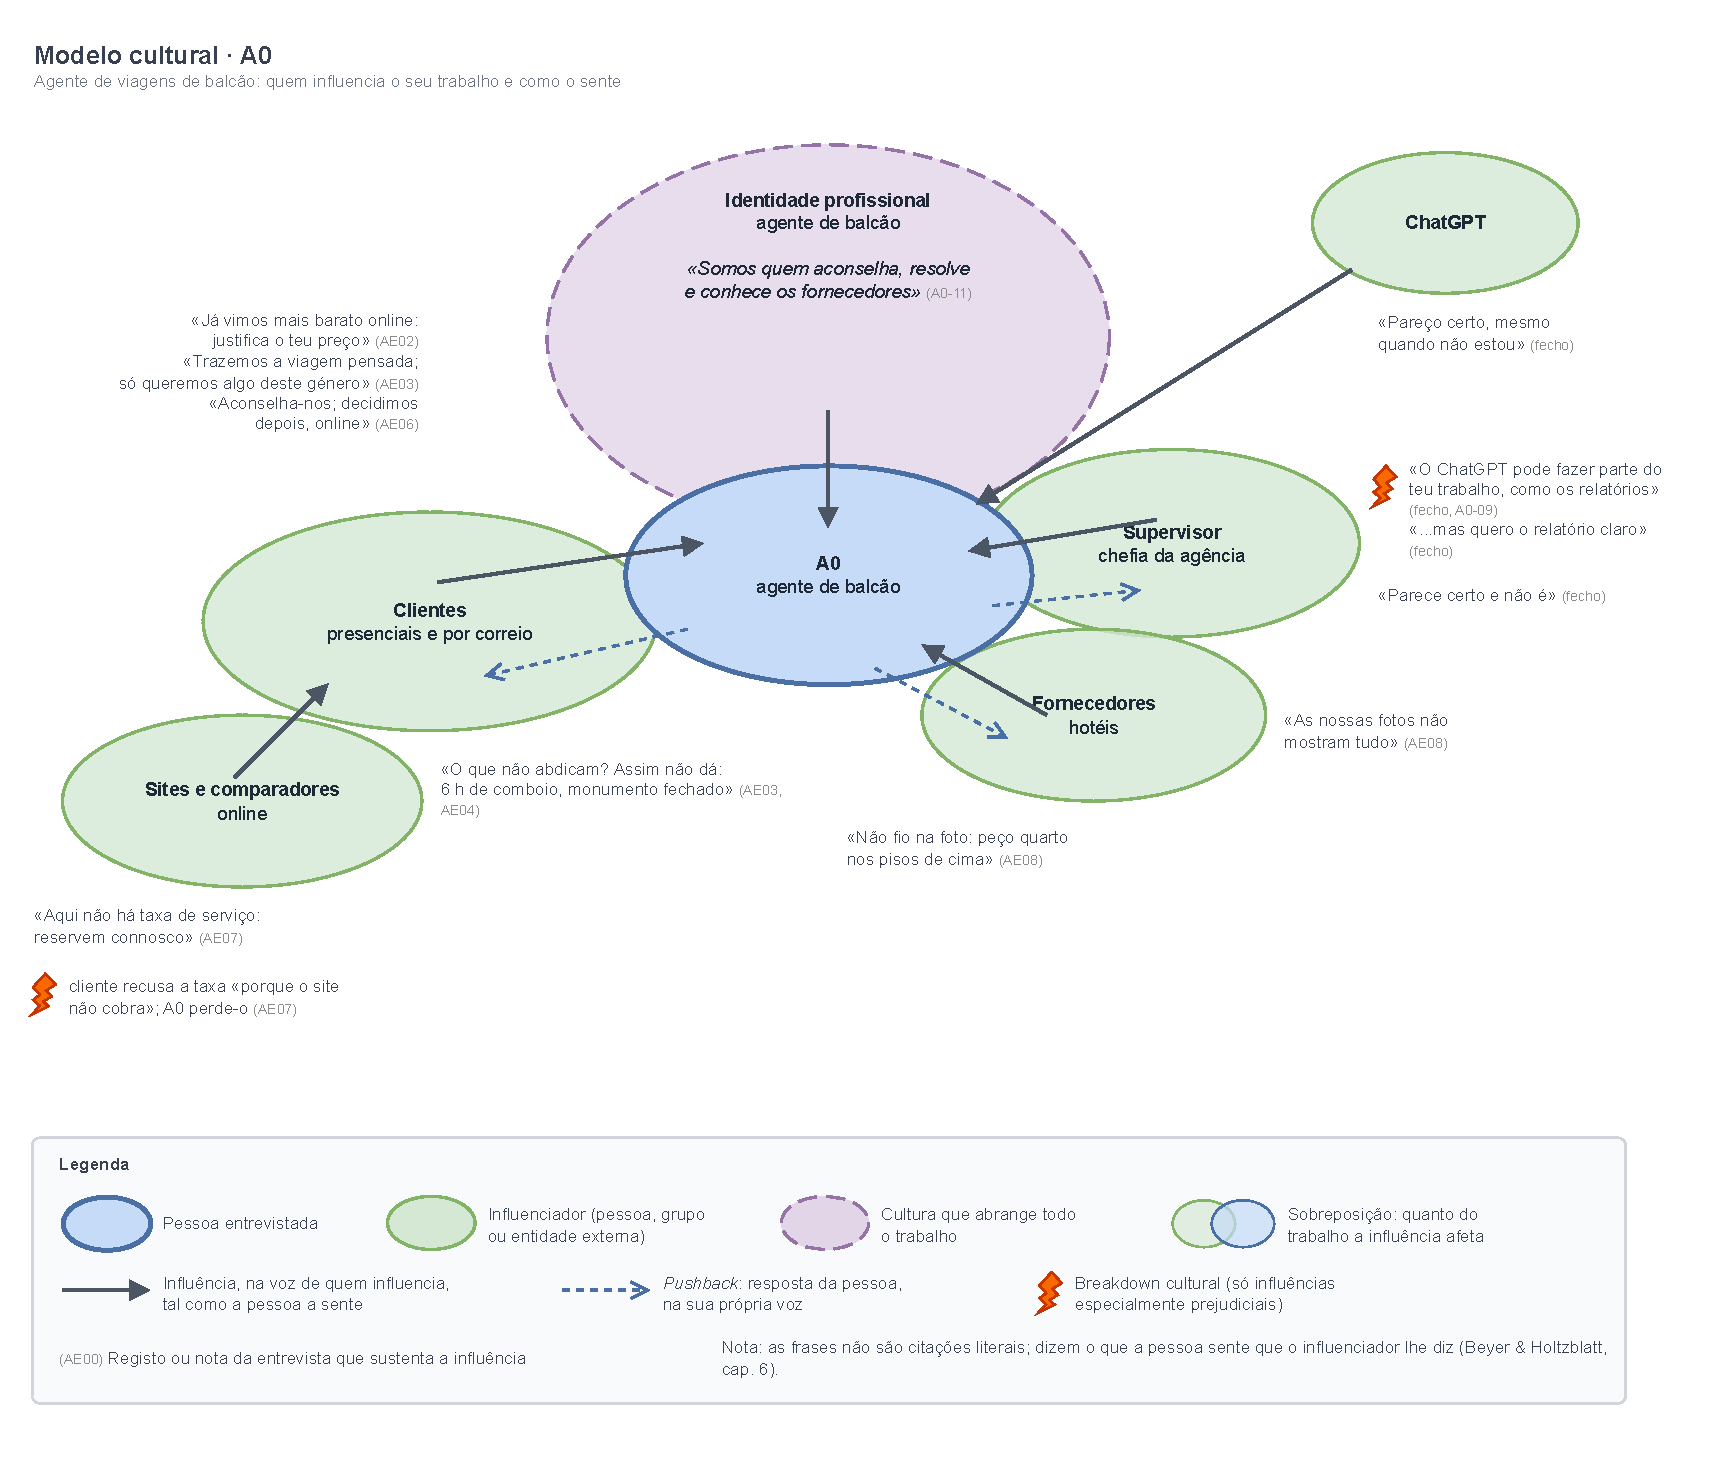
\includegraphics[width=\textwidth]{cultural_models/individuais/CulturalA0.drawio.pdf}
\caption{Modelo cultural de A0 (agente de viagens de balcão).}
\label{fig:cultural-a0}
\end{figure}

A identidade profissional pesa sobre todo o trabalho de A0: 
«somos quem aconselha, resolve e conhece os fornecedores» \reg{A0-11}. 
As influências mais fortes vêm dos \textbf{clientes}, que chegam com a 
viagem pensada e usam os preços online como pressão \reg{AE02, AE03, AE06}. 
Por trás deles estão os \textbf{sites e comparadores}, que não cobram taxa de serviço; 
essa influência chega a A0 através do cliente que recusa a taxa e se perde \reg{AE07}. 
O \textbf{supervisor} acha que o ChatGPT pode fazer parte do trabalho de A0, como 
redigir os relatórios, embora não goste quando o relatório sai confuso \reg{A0-09}, 
e o próprio \textbf{ChatGPT} é sentido como uma ferramenta que «parece certa, 
mesmo quando não está». A0 resiste: aponta ao cliente o que é inviável e diz ao 
supervisor que a IA «parece certa e não é».

\begin{table}[!htbp]
\centering\small
\begin{tabularx}{\textwidth}{@{}p{0.5cm}Lp{2.6cm}@{}}
\toprule
 & \textbf{Influência especialmente prejudicial} & \textbf{Registo} \\
\midrule
\bolt & Sites sem taxa de serviço levam o cliente a recusar a taxa; A0 perde o cliente. & AE07 \\
\bolt & O supervisor acha que o ChatGPT pode fazer parte do trabalho de A0 (os relatórios). & Fecho, A0-09 \\
\bottomrule
\end{tabularx}
\caption{\textit{Breakdowns} do modelo cultural de A0.}
\label{tab:bd-cult-a0}
\end{table}

\subsubsection{Cultural de U0}

\begin{figure}[!htbp]
\centering
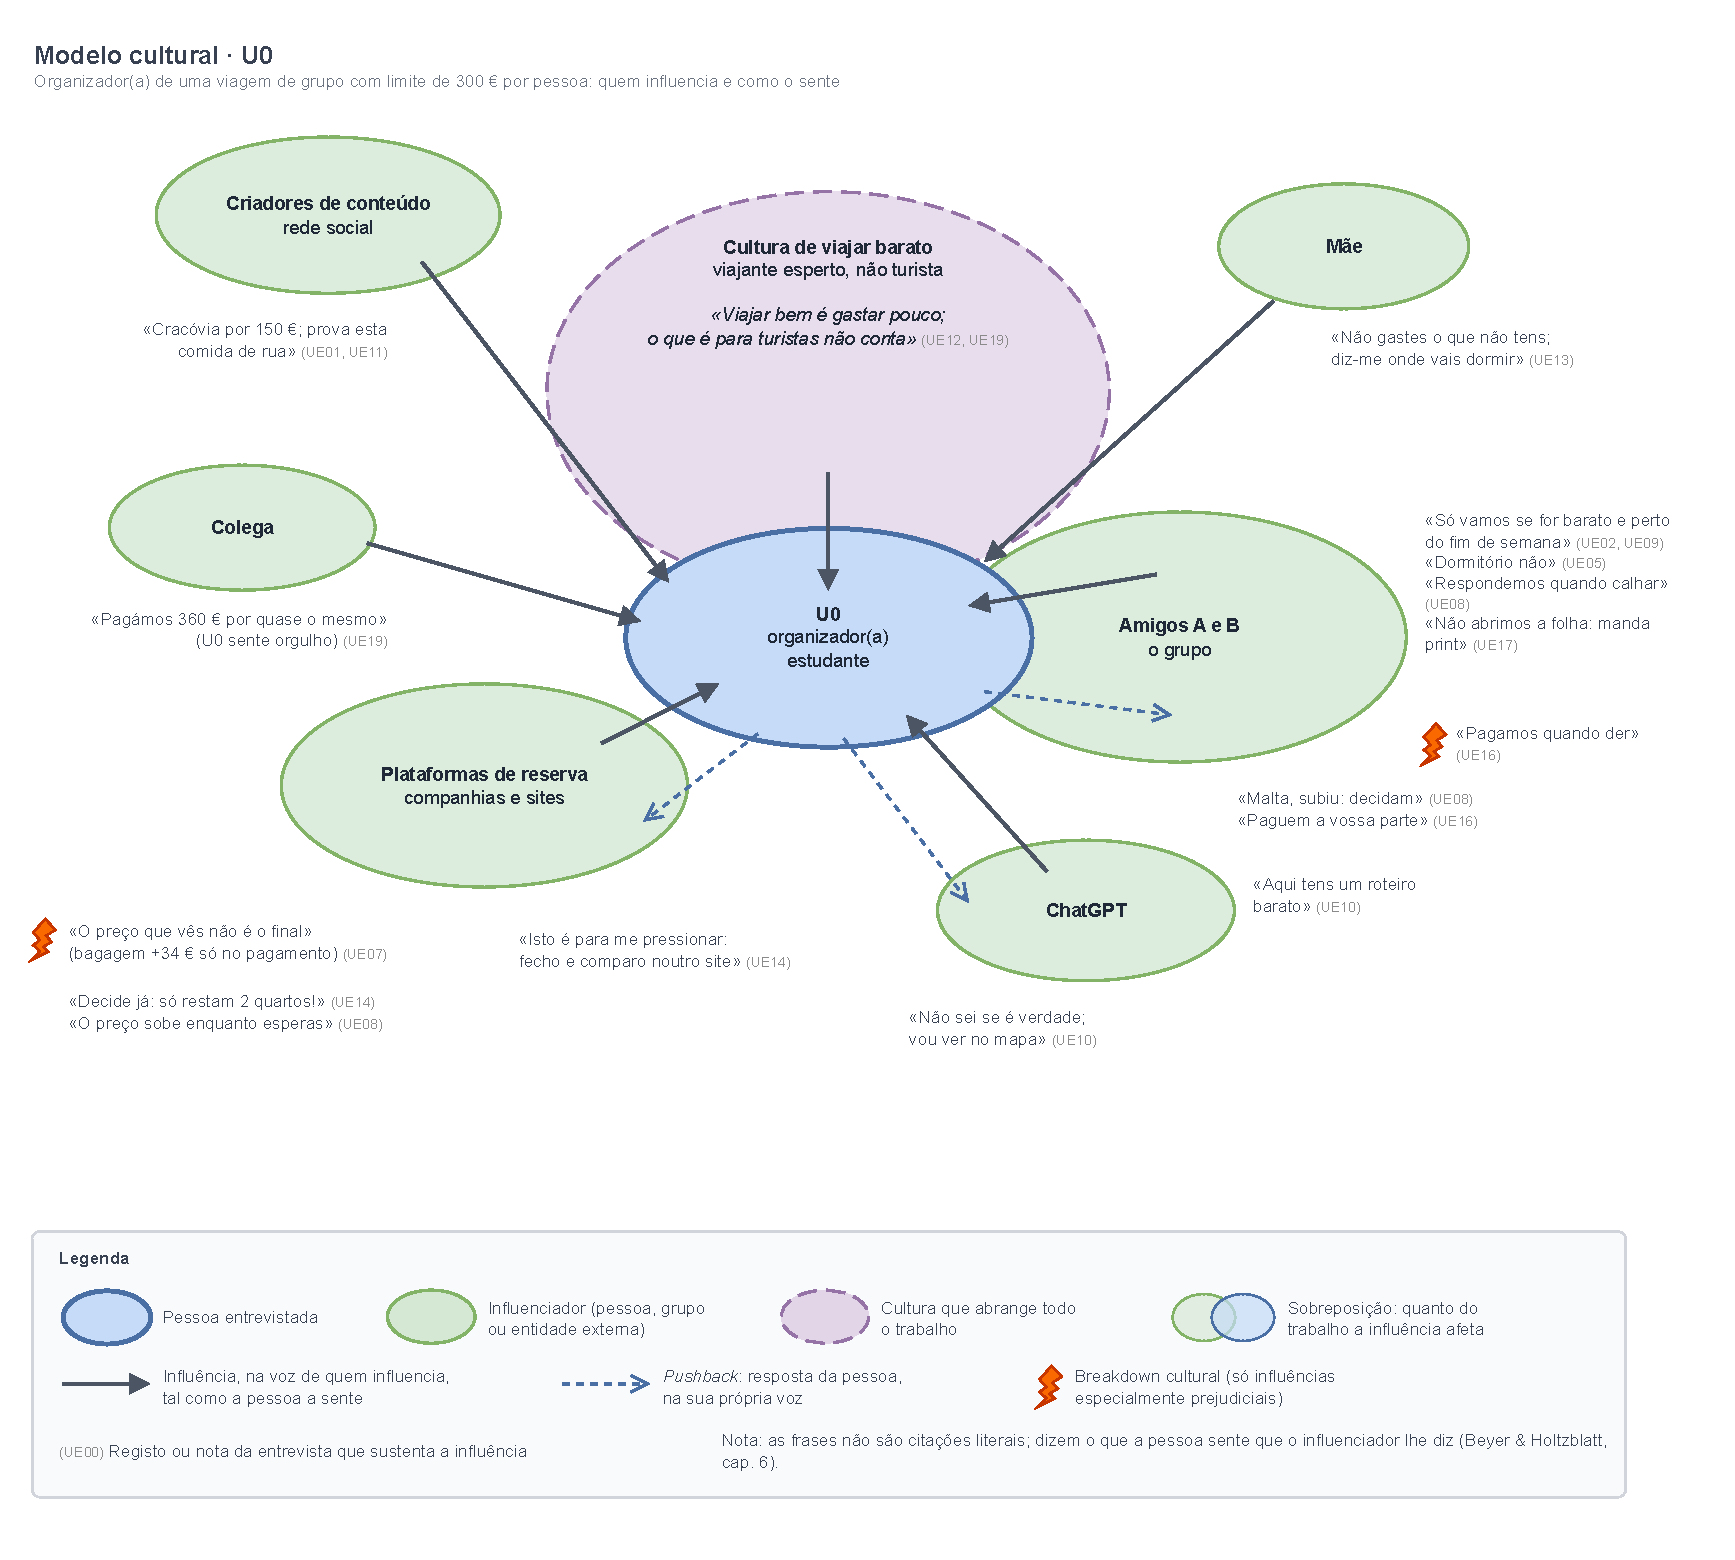
\includegraphics[width=\textwidth]{cultural_models/individuais/CulturalU0.drawio.pdf}
\caption{Modelo cultural de U0 (viajante organizador).}
\label{fig:cultural-u0}
\end{figure}

U0 vive dentro de uma \textbf{cultura de viajar barato}: «viajar bem é gastar pouco; 
o que é para turistas é armadilha». É ela que justifica cortar a mina de sal \reg{UE12} 
e que dá orgulho em pagar menos do que uma colega \reg{UE19}. Os \textbf{amigos} são 
a influência com mais peso: condicionam as datas e o tipo de alojamento, respondem 
devagar e pagam tarde \reg{UE02, UE05, UE08, UE16, UE17}. As 
\textbf{plataformas de reserva} são sentidas como adversárias: 
escondem custos e pressionam com «só restam 2 quartos!» \reg{UE07, UE14}. 
U0 resiste: fecha o separador e compara noutro site, pede ao grupo que 
decida e pague, e verifica no mapa o que o ChatGPT sugere \reg{UE08, UE10, UE14, UE16}. 
A \textbf{mãe} e os \textbf{criadores de conteúdo} têm influências mais 
pontuais \reg{UE01, UE11, UE13}.

\begin{table}[!htbp]
\centering\small
\begin{tabularx}{\textwidth}{@{}p{0.5cm}Lp{2.6cm}@{}}
\toprule
 & \textbf{Influência especialmente prejudicial} & \textbf{Registo} \\
\midrule
\bolt & As plataformas mostram um preço que não é o final (bagagem só no pagamento). & UE07 \\
\bolt & O grupo paga «quando der»: U0 fica a fazer de banco. & UE16 \\
\bottomrule
\end{tabularx}
\caption{\textit{Breakdowns} do modelo cultural de U0.}
\label{tab:bd-cult-u0}
\end{table}

%----------------------------------------------------------
\subsection{Modelos de sequência}\label{sec:sequencia}

%----------------------------------------------------------
\subsection{Modelos de artefacto}\label{sec:artefacto}

%----------------------------------------------------------
\subsection{Modelos físicos}\label{sec:fisico}
